The InStream component models the interface through which packets representing incoming commands or reports are received by an application. The InStream component is therefore located at the interface between an application and the middleware layer (see section \ref{sec:MwLayer}). 

An application A may receive packets from several sources. The packets may either have application A as their destination or they may be intended for some other application. In the latter case, application A is responsible for re-routing the packets. Depending on the characteristics of the middleware, only one InStream component may be present in application A with the multiplexing of the incoming connections from the packet sources being done in the middleware, or several InStream components may be present each handling packets from a subset of incoming connections. 

Although several connections may be managed by the same InStream, a connection can only send its packet to one InStream (i.e. a situation where the same connection is controlled by several InStreams and several InStreams are therefore handling packets from the same source is not allowed).

The InStreams are responsible for checking the sequence counter attributes of incoming packets received by an application. Since sequence counters are incremented according to a packet's group, all packets belonging to the same group must arrive through the same InStream.

The InStream component is defined as an extension of the Base Component of section \ref{sec:BaseCmp} and it therefore inherits the initialization and configuration logic defined by the Base Component. In the initialization and configuration process, the InStream is linked to the middleware. This process is therefore necessarily application-specific (because the middleware is not specified by the CORDET Framework). However, the CORDET Framework specifies that an InStream component may only become configured (i.e. it may enter state CONFIGURED) after the middleware connection has terminated its own initialization and configuration. This ensures that an InStream only becomes configured after its middleware connection has terminated its own initialization and configuration process.

\begin{figure}[ht]
 \centering
 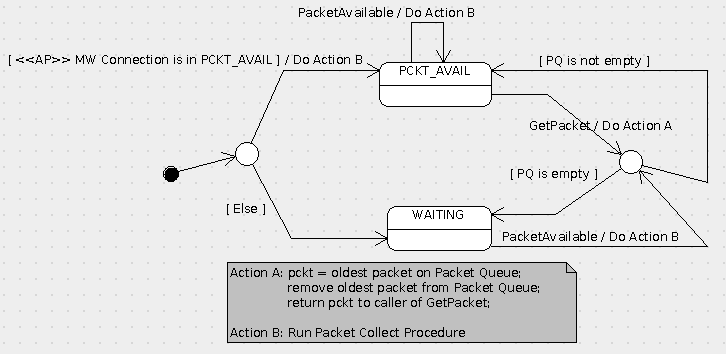
\includegraphics[scale=0.45,keepaspectratio=true]{InStream.png}
 \caption{The InStream State Machine}
 \label{fig:InStream}
\end{figure}

\begin{figure}[h]
 \centering
 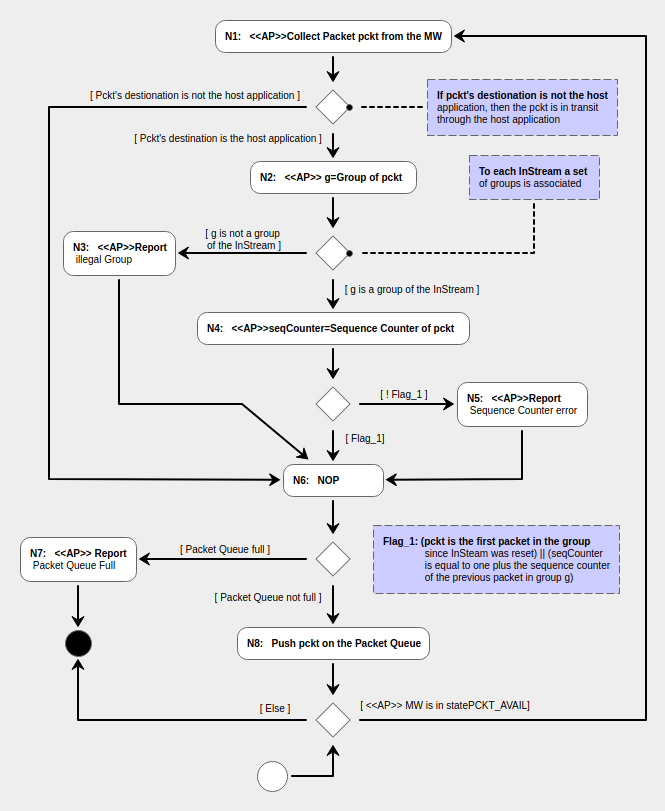
\includegraphics[scale=0.45,keepaspectratio=true]{PacketCollect.png}
 \caption{The Packet Collect Procedure}
 \label{fig:PacketCollect}
\end{figure}

In state CONFIGURED, the behaviour of an InStream is described by the state machine of figure \ref{fig:InStream} (the \textit{InStream State Machine}). The state machine has two states: WAITING and PCKT\_AVAIL. State WAITING represents a situation where no incoming packets are waiting to be collected by the host application. State PCKT\_AVAIL represents a situation where at least one incoming packet has been collected from the middleware and is now waiting to be collected by the host application. 

The InStream component stores packets it has collected from the middleware in the \textit{Packet Queue}. The Packet Queue is an internal InStream data structure where packets which have been collected from the middleware are stored and where they remain available until the application retrieves them. The size of the packet queue is fixed and is defined as part of the InStream configuration. Attempts to enqueue a packet in a full queue are reported as errors.

The Packet Queue is a FIFO queue. This guarantees that the InStream component delivers packets to its host application in the same order in which it has collected them from the middleware. The InStream State Machine reacts to two commands: \texttt{GetPacket} and \texttt{PacketAvailable}. Command \texttt{GetPacket} is issued by the host application when it wishes to collect an incoming packet. If the command is received when the state machine is in state PCKT\_AVAIL (namely when at least one packet is available in the Packet Queue), then the command results in the oldest packet in the Packet Queue being returned to the caller. If the packet thus returned is the last on the queue, the command triggers a transition to state WAITING. 

If the \texttt{GetPacket} command is received when the state machine is in state WAITING, the command has no effect and returns nothing.

Command \texttt{PacketAvailable} would typically be issued under two conditions: (a) in response to the middleware connection changing from NOT\_AVAIL to AVAIL, or (b) periodically to check whether any packets are available at the middleware interface. Case (a) corresponds to a call-back architecture where the middleware alerts the application that a new packet has arrived. Case (b) corresponds to a polling architecture where the application periodically checks whether a new packet has arrived. 

Reception of command \texttt{PacketAvailable} causes the \textit{Packet Collect Procedure} of figure \ref{fig:PacketCollect} to be run. This procedure collects all packets currently available at the middleware. The packets are stored in the InStream's Packet Queue. 

Also as part of the processing of the \texttt{PacketAvailable} command, the \textit{Packet Collect Procedure} checks the sequence counter attribute of incoming packets which have the host application as their destination. Each packet belongs to a \textit{group} (see sections \ref{sec:CmdAttributes} and \ref{sec:RepAttributes}). When a packet is received which belongs to a certain group, the Packet Collect Procedure checks that its sequence counter has incremented by one with respect to the previous packet in the same group. If the procedure finds that the sequence counter has not incremented by one, it reports the sequence counter error. An error is also reported if the group attribute of an incoming packet does not correspond to one of the groups managed by the InStreams.

The sequence counter check is only done for packets which have the host application as their destinations. Packets which are in transit (i.e. packets which must be re-routed to some other application) do not undergo any check on their sequence counter. This logic ensures that the sequence counter check is only performed once by the InStream that receives a packet in the destination application of that packet. 
